\begin{center}
\large{\textbf{Information and Bargaining through Agents: Experimental Evidence from Mexico's Labor Courts}}

%\shortTitle{Information and Bargaining through Agents}

\textit{Joyce Sadka,  Enrique Seira, and Christopher Woodruff}

\Large{\textbf{Online Appendices}}
\end{center}

\section*{Appendix A}
\label{appendix_a}
\title{\Large{\textbf{Mexican Labor Law, Description of Data, and the Calculator}}}
\\

\setcounter{table}{0}
\renewcommand{\thetable}{A.\arabic{table}} 
\setcounter{figure}{0}
\renewcommand{\thefigure}{A.\arabic{figure}} 

The appendix is divided into four sections. The first describes the Mexican labor law and court procedures, the second provides some additional details on the administrative data, the third describes our surveys and response rates, and the fourth describes the calculator we use to make predicted outcomes for the cases in which we intervene. 

\subsection{Mexican Labor Law}

\textbf{Mexican labor Law:} On paper, Mexican labor law is protective of workers. For any employer-initiated separation that is not a '`justified dismissal,'' the law requires severance payment of a minimum of 90 days' wages and benefits. The law provides very few legal bases for a justified dismissal. For example, workers are owed severance if they are fired for low productivity or because of poor market conditions.  As an element of their lawsuit, workers may ask the court to order the firm to rehire them. If they win their case and the firm refuses to rehire them, then they are entitled to an additional severance payment equal to 20 days' wages for each year of tenure at the firm.\footnote{Certain categories of workers (those defined as '`at-will'') are also entitled to to 20 days' wages per year of tenure. An at-will worker is one who is employed in a position of confidence, for example, a driver or a personal security guard. The law recognizes that the employer may need to dismiss the worker if that confidence is broken.} 

\textbf{The Process:} In a firing lawsuit, an initial claim is filed by the worker or her lawyer, and an initial hearing date is set, generally two to three months after the date of filing. The defendant(s) must be notified of the filing and hearing date by a formal court summons that must be delivered in person by an employee of the court. The notification process typically takes 6 months.\footnote{In practice, notification involves substantial corruption, as the lawsuit cannot proceed without it.  \cite{KaplanSadka_notif} shows that when notifiers' work load is assigned randomly and control of case files is taken away from notifiers, rates of successful notification more than double.} Once notification of all defendants has taken place, a '`conciliation, demands, and answers'' hearing takes place. The principal demand in most firing lawsuits is either the base severance pay of 90 days or reinstatement of employment. 

If a settlement cannot be reached then the defendant must answer the lawsuit. Additional hearings are scheduled for presentation and viewing of evidence, after which the written record is closed. All proceedings are conducted by an administrative assistant to the judge. Hearings are transcribed into the case file. The file is passed on to the judge, who writes the final decision. Enforcement of judgments involving payments to the plaintiff is often challenging. A large proportion of firms do not pay the judgment voluntarily, and a seizure of assets must officially be performed by officers of the court. This is  followed by adjudication of liquid assets or sale of non-liquid assets to pay the worker the awarded amount. Given that an interval of six-months between hearings is typical, the fact that there are more than four hearings held in an average case, and the frequent postponement of scheduled hearings due to lack of notification, the average lawsuit continuing to a judge's decision takes over three years. This in spite of the law stipulating that lawsuits should have a maximum duration of 100 days. 

\textbf{Lawyers:} Once a case is filed, lawyers control the lawsuits almost completely. The presence of the parties themselves at the hearings is not compulsory, unless they are to be deposed as part of the evidentiary hearings. By law, workers who are not able to hire a private lawyer must be provided with free public legal assistance from labor lawyers in the public prosecutor's office. Public lawyers are paid a flat wage by the court and may not charge  clients anything further. A public lawyer handles as many as 400 cases concurrently, while administrative data suggest that a normal load for a private lawyer is at most 50 cases. So while public lawyers are generally well qualified, they have an incentive to finish cases quickly in order to reduce their workload. The general perception is that public lawyers do not use creative or aggressive litigation strategies that may have a positive payoff but imply longer cases or more work. 

Private lawyers must be licensed, but obtaining the license is fairly easy and otherwise lawyers are unregulated. Survey data indicate that 82 percent of workers are suing for the first time. Workers have little access to information about where to find a good private lawyer, and often opt for the first one that they run into, with little notion of that lawyer's reputation or previous record. The surveys show that 38 percent of plaintiffs using a private lawyer say that they found the lawyer either just outside the court or in one of the court corridors. Plentiful anecdotal evidence suggests that these '`informal lawyers'' are low-quality and may not serve their clients' best interests. 

Private plaintiff's lawyers typically charge an initial fee of about MXN\$2000 pesos (USD 100) to file the lawsuit and a contingency fee of about 30 percent of any amount collected by the plaintiff. In spite of the contingency fee, their incentives are not perfectly aligned to those of their clients. First, while plaintiffs are party to a single case, the lawyers manage a portfolio of many firing lawsuits with widely differing characteristics, against many different firms. With diversified risk, they may be more willing to take risks on any given case.   Second, filing a low-quality suit is cheap and easy and the lawyers may profit from collecting the filing fee even with no expectation of recovering anything on behalf of the worker.  The plaintiff must ratify settlements of the lawsuit in person, as well as acceptance or rejection of an offer of reinstatement, should the plaintiff's side receive one. Lawyers typically do not bring the plaintiffs to hearings nor do they provide them much detail on the developments in the lawsuit. As will be shown below, the physical presence of the worker at the hearing in which we intervene in the field experiment is crucial for the effectiveness of our intervention. 

 %\footnote{Private lawyers may have incentives to convince a worker to sue and not settle even when it is not in her interest to do so. The most common way of doing this is to inflate the claim by adding elements to it, even if in the end they won't stand up in court (e.g. lost wages, vacation pay, end of year bonus, and overtime), and by exaggerating the worker's salary, which is often paid by the firm totally or partially in an informal way.}
 
 \FloatBarrier
 
\subsection{Administrative Data}

The main source of administrative data are the initial case filings for the historical and experimental cases. For the experimental cases, we also collected data on the phase 1 and 2 case outcomes in December 2018 and in January and July  2020. The historical data are used to develop a predictive model of case outcomes. We then use this model and the data from each experimental case filing to predict outcomes for each case, as described in subsection \ref{calculator_method} below. Because we intervene in many cases at the time of their first hearing, we use only data from the initial case filing. The case files are available in hard copy, and we digitize the variables shown on Table \ref{variable_list}. 

\begin{table}[!ht]
    \caption{Casefile Variable}
    \label{variable_list}
    \begin{center}
        \scriptsize{% Table generated by Excel2LaTeX from sheet 'Variable_list'
\begin{tabular}{p{2.25cm}| p{12cm}}
\toprule
\rowcolor[rgb]{ .267,  .329,  .416} \textcolor[rgb]{ 1,  1,  1}{\textbf{VARIABLE}} & \textcolor[rgb]{ 1,  1,  1}{\textbf{DESCRIPTION}} \\
\midrule
\textbf{Tenure} & Employee's tenure with the employer. \\
\midrule
\textbf{Weekly hours} & Number of hours that the plaintiff worked on a weekly basis. \\
\midrule
\textbf{Reinstatement*} & The plaintiff claims reinstatement. \\
\midrule
\textbf{Severance pay*} & The plaintiff claims constitutional indemnity (three months of integrated salary) that the law dictates for unjustified dismissal. \\
\midrule
\textbf{Lost wages*} & The plaintiff claims lost wages/back pay. \\
\midrule
\textbf{Vacation pay*} & The plaintiff claims accrued vacation days not taken. \\
\midrule
\textbf{Overtime*} & The plaintiff claims overtime pay. \\
\midrule
\textbf{Twenty days compensation*} & The plaintiff claims the payment of compensation (20 days per year worked) that the law dictates for unjustified dismissal for a worker who has the right to be reinstated but the employer refuses to reinstate, or for an at-will employee who cannot ask for reinstatement. \\
\midrule
\textbf{Insurance- IMSSINFOSAR*} & The plaintiff claims the payment of employer contributions that were not made to these institutions, or retroactive registration in the institutions (SAR: retirement savings, IMSS: social security, INFONAVIT: worker's housing fund). \\
\midrule
\textbf{Co-defendant*} & At least one of the codefendants is the IMSS or INFONAVIT or SAR. \\
\midrule
\textbf{Total asked} & The total quantifiable peso amount of the worker's claim. \\
\midrule
\textbf{Minimum legal entitlement} & The quantifiable peso amount of the sum of severance pay, vacation and end of year bonuses of the last year of tenure at the firm. It is a conservative estimate of the minimum amount of money the worker is entitled to if she wins the lawsuit. \\
\bottomrule
\end{tabular}%
}
    \end{center}
     \scriptsize
    \textit{Notes:} 
Detailed description of variables used throughout the paper. Dummy variables are marked with \textbf{*}.
\end{table}


\FloatBarrier

\subsection{Survey Data}

We conducted surveys with participants at the hearings in Phases 1 and 2, and with dismissed workers approaching the court in Phase 3. The surveys in the first two phases had to be very short so that we did not delay the start of hearings. We use one survey instrument for plaintiffs, and another for the lawyers representing both plaintiffs and employers. Table \ref{ss_survey} shows summary statistics for workers and lawyer from phase 1. Table \ref{Table_compliance} shows compliance rates for both the surveys and treatments for the first two phases. We have no measure of noncompliance in phase 3. Every worker who completed the survey and was assigned to treatment received the calculator treatment. However, there were surely dismissed workers who approached the court but did not stop at our information booth. Since the workers approaching the court had no way of know if the given day was assigned to treatment or control, we have no reason to believe there is differential non-compliance across treatment groups on either observable or unobservable characteristics. Hence, non-compliance in phase 3 is an issue of external rather than internal validity.\footnote{Even if every dismissed worker approaching the court had fully complied with the experimental protocol, the sample would not be representative of all aggrieved workers dismissed from Mexico City employers, because many dismissed workers obtain information from public or private lawyers without coming to the court. However, we believe the sample is relevant for understanding the effect of information provision on the decision to file case or settle.}  

\begin{table}[!ht]
     \caption{Survey variables summary statistics}
     \label{ss_survey}
     \begin{center}
     \resizebox{16.5cm}{!}{
     \scriptsize{% Table generated by Excel2LaTeX from sheet 'surveySS'
\begin{tabular}{rrcccc}
\toprule
\multicolumn{6}{c}{\textbf{Panel A: worker characteristics}} \\
\midrule
      &       & Mean  &       &       & Mean \\
      &       & (SD)  &       &       & (SD) \\
      &       & N     &       &       & N \\
\midrule
\multicolumn{2}{l}{Age} & 44.4 & \multicolumn{2}{l}{More than secondary education} & 0.42 \\
\multicolumn{2}{r}{} & (13.2) & \multicolumn{2}{r}{} & (0.50) \\
\multicolumn{2}{r}{} & 102   & \multicolumn{2}{r}{} & 102 \\
\multicolumn{2}{l}{Firm had less than 50 employees} & 0.59  & \multicolumn{2}{l}{Was treated poorly/very poorly by former employer} & 0.55  \\
\multicolumn{2}{r}{} & (0.49) & \multicolumn{2}{r}{} & (0.50) \\
\multicolumn{2}{r}{} & 96    & \multicolumn{2}{r}{} & 102 \\
\multicolumn{2}{l}{Expected probability of winning trial} & 79.0   & \multicolumn{2}{l}{Mean / Median expected recovery (Pesos)} & 97,116 / 21,000 \\
\multicolumn{2}{r}{} & (21.3) & \multicolumn{2}{r}{} & (355,749) \\
\multicolumn{2}{r}{} & 102    & \multicolumn{2}{r}{} & 102 \\
\multicolumn{2}{l}{What would employer report as probability of winning?} & 48.7 & \multicolumn{2}{l}{Expected duration (years)} & 3.64 \\
\multicolumn{2}{r}{} & (34.1) & \multicolumn{2}{r}{} & (9.76) \\
\multicolumn{2}{r}{} & 102   & \multicolumn{2}{r}{} & 102 \\
\multicolumn{2}{l} {Percentage paid to lawyer} & 28.3  & \multicolumn{2}{l} {Has changed lawyer during trial} & 0.09 \\
\multicolumn{2}{r}{} & (11.1) & \multicolumn{2}{r}{} & (0.29) \\
\multicolumn{2}{r}{} & 57   & \multicolumn{2}{r}{} & 102 \\
\multicolumn{2}{r}{} &       & \multicolumn{2}{r}{} &  \\
\midrule
\midrule
\multicolumn{6}{c}{\textbf{Panel B: lawyer characteristics}} \\
\midrule
      &       & \multicolumn{2}{c}{Worker's lawyer} & \multicolumn{2}{c}{Employer's lawyer} \\
\midrule
      &       & \multicolumn{2}{c}{Mean} & \multicolumn{2}{c}{Mean} \\
      &       & \multicolumn{2}{c}{(SD)} & \multicolumn{2}{c}{(SD)} \\
\multicolumn{2}{r}{} & \multicolumn{2}{c}{N} & \multicolumn{2}{c}{N} \\
\midrule
\multicolumn{2}{l}{Age} & \multicolumn{2}{c}{37.8} & \multicolumn{2}{c}{36.6} \\
\multicolumn{2}{r}{} & \multicolumn{2}{c}{(12.4)} & \multicolumn{2}{c}{(11.0)} \\
\multicolumn{2}{r}{} & \multicolumn{2}{c}{231} & \multicolumn{2}{c}{223} \\
\multicolumn{2}{l}{Tenure} & \multicolumn{2}{c}{9.25} & \multicolumn{2}{c}{18.7} \\
\multicolumn{2}{r}{} & \multicolumn{2}{c}{(8.88)} & \multicolumn{2}{c}{(143.3)} \\
\multicolumn{2}{r}{} & \multicolumn{2}{c}{181} & \multicolumn{2}{c}{193} \\
\multicolumn{2}{l}{More than 100 historical cases} & \multicolumn{2}{c}{0.49} & \multicolumn{2}{c}{0.61} \\
\multicolumn{2}{r}{} & \multicolumn{2}{c}{(0.50)} & \multicolumn{2}{c}{(0.49)} \\
\multicolumn{2}{r}{} & \multicolumn{2}{c}{231} & \multicolumn{2}{c}{223} \\
\multicolumn{2}{l}{More than 30 current lawsuits} & \multicolumn{2}{c}{0.60} & \multicolumn{2}{c}{0.68} \\
\multicolumn{2}{r}{} & \multicolumn{2}{c}{(0.49)} & \multicolumn{2}{c}{(0.47)} \\
\multicolumn{2}{r}{} & \multicolumn{2}{c}{231} & \multicolumn{2}{c}{223} \\
\multicolumn{2}{l}{Less than 50 employees} & \multicolumn{2}{c}{0.65} & \multicolumn{2}{c}{0.46} \\
\multicolumn{2}{r}{} & \multicolumn{2}{c}{(0.48)} & \multicolumn{2}{c}{(0.50)} \\
\multicolumn{2}{r}{} & \multicolumn{2}{c}{173} & \multicolumn{2}{c}{151} \\
\multicolumn{2}{l}{Percentage paid to lawyer} & \multicolumn{2}{c}{29.7} & \multicolumn{2}{c}{} \\
\multicolumn{2}{r}{} & \multicolumn{2}{c}{(7.79)} & \multicolumn{2}{c}{} \\
\multicolumn{2}{r}{} & \multicolumn{2}{c}{172} & \multicolumn{2}{c}{} \\
\multicolumn{2}{l}{Expected probability of winning trial} & \multicolumn{2}{c}{72.2} & \multicolumn{2}{c}{70.5} \\
\multicolumn{2}{r}{} & \multicolumn{2}{c}{(20.1)} & \multicolumn{2}{c}{(21.5)} \\
\multicolumn{2}{r}{} & \multicolumn{2}{c}{231} & \multicolumn{2}{c}{223} \\
\multicolumn{2}{l}{Mean / Median expected recovery (Pesos)} & \multicolumn{2}{c}{237,958 / 35,000} & \multicolumn{2}{c}{66,885 / 11,000} \\
\multicolumn{2}{r}{} & \multicolumn{2}{c}{(1,482,120)} & \multicolumn{2}{c}{(285,657)} \\
\multicolumn{2}{r}{} & \multicolumn{2}{c}{231} & \multicolumn{2}{c}{223} \\
\multicolumn{2}{l}{Expected duration (years)} & \multicolumn{2}{c}{3.94} & \multicolumn{2}{c}{4.17} \\
\multicolumn{2}{r}{} & \multicolumn{2}{c}{(2.30)} & \multicolumn{2}{c}{(2.54)} \\
\multicolumn{2}{r}{} & \multicolumn{2}{c}{231} & \multicolumn{2}{c}{223} \\
\bottomrule
\bottomrule
\end{tabular}%
}
     }
     \end{center}
     \scriptsize
     \textit{Notes:} Summary statistics of survey variables for Pilot 1 participants. The parties were surveyed before the case. The plaintiff was surveyed if present and the plaintiff's lawyer was surveyed otherwise. The firm was almost never present, so the lawyer was surveyed from the defendant's side. The number of responses varies across questions due to item non-responses. 
 \end{table}
 % Do file: surveyP1SS.do

\begin{landscape}
\begin{table}[!ht]
    \caption{Compliance Rate}
    \label{Table_compliance}
    \begin{subtable}{1\textwidth}
      \centering
        \caption{Phase 1}
        \scriptsize{% Table generated by Excel2LaTeX from sheet 'Compliance'
\begin{tabular}{lrcccccccccccc}
\toprule
\multicolumn{1}{c}{Group} & \multicolumn{1}{c}{N} & \multicolumn{4}{c}{Compliance with treatment} & \multicolumn{4}{c}{Compliance with baseline survey} & \multicolumn{4}{c}{Compliance with exit survey} \\
\midrule
\midrule
      &       & Plaintiff & Defendant & Both  & Any   & Plaintiff & Defendant & Both  & Any   & Plaintiff & Defendant & Both  & Any \\
\midrule
Control & 321   & -     & -     & -     & -     & 50.78 & 35.51 & 8.72  & 77.57 & 39.88 & 24.3  & 5.61  & 58.57 \\
Calculator & 315   & 77.65 & 73.03 & 75.81 & 79.72 & 48.25 & 33.65 & 12.38 & 69.52 & 38.63 & 25.86 & 9.66  & 54.83 \\
\bottomrule
\end{tabular}%
}
    \end{subtable}%
    
    \bigskip
    \begin{subtable}{1\textwidth}
      \centering
        \caption{Phase 2}
        \scriptsize{% Table generated by Excel2LaTeX from sheet 'complianceP2'
\begin{tabular}{lrrrrrrrrr}
\toprule
Group & \multicolumn{1}{l}{N} & \multicolumn{4}{c}{Compliance with treatment} & \multicolumn{4}{c}{Compliance with survey} \\
\midrule
\midrule
      &       & \multicolumn{1}{l}{Plaintiff} & \multicolumn{1}{l}{Defendant} & \multicolumn{1}{l}{Both} & \multicolumn{1}{l}{Any} & \multicolumn{1}{l}{Plaintiff} & \multicolumn{1}{l}{Defendant } & \multicolumn{1}{l}{Both } & \multicolumn{1}{l}{Any} \\
\midrule
\midrule
Control & 329   & \multicolumn{1}{l}{-} & \multicolumn{1}{l}{-} & \multicolumn{1}{l}{-} &       & \multicolumn{1}{l}{-} & \multicolumn{1}{l}{-} & \multicolumn{1}{l}{-} & \multicolumn{1}{l}{-} \\
Calculator & 762   & 72.7  & 63.78 & 49.08 & 87.4  & 54.33 & 48.29 & 49.08 & 87.4 \\
\bottomrule
\end{tabular}%
}
    \end{subtable}
    
      \bigskip
    \begin{subtable}{1\textwidth}
      \centering
        \caption{\% Shows up}
        \scriptsize{% Table generated by Excel2LaTeX from sheet 'show_up'
\begin{tabular}{lcccc}
\toprule
      & \multicolumn{2}{c}{Phase 1} & \multicolumn{2}{c}{Phase 2} \\
\midrule
\midrule
      & Control & Calculator & Control & Calculator \\
\midrule
\midrule
\multicolumn{1}{p{4.055em}}{Employee } & 0.193 & 0.197 & 0.122 & 0.165 \\
Emp Lawyer & 0.847 & 0.832 & 0.85  & 0.853 \\
Firm Lawyer & 0.738 & 0.762 & 0.434 & 0.444 \\
\bottomrule
\bottomrule
\end{tabular}%
}
    \end{subtable}
            \scriptsize
           \\
           \\
           \\
  \textit{Notes:} 
  Compliance rate for each phase, both for treatment and survey. Each panel shows the percentage compliance with treatment and survey for plaintiff' side, defendant's side, both, and any. In phase 1, we did not measure compliance with treatment at the party level but rather at the casefile level, so that for example the 74.16 under the column "both" for compliance with treatment means that among the casefiles for which both parties showed up to the hearing, we were able to give the calculator to at least one of the parties in 74.16 percent of the cases. Also, in phase 1 we had an exit survey in addition to the baseline survey. In phase 2, we did measure compliance with the treatment by party. On the other hand, note from panel (b) that since in phase 2 control days were days that no implementing personnel were present in the subcourts, we have neither treatment nor survey compliance for the control group. Panel (c) shows from the court's administrative data who shows up to the hearings for each of the two phases, split by employee, employee lawyer, and firm lawyer.
    % \textit{Scripts: } \texttt{complianceTable.do, ComplianceP2Tables.do, showUp.do}
\end{table}
\end{landscape}







\begin{table}[!ht]
  \caption{Balance table}
    \label{balance_table}
    \begin{center}
    \scriptsize{% Table generated by Excel2LaTeX from sheet 'Balance'
\begin{tabular}{lccccccccc}
\toprule
      & \multicolumn{3}{c}{Phase 1} & \multicolumn{3}{c}{Phase 2} & \multicolumn{2}{c}{Phase 1/2} &  \\
\midrule
\midrule
      & C     & T     & p-value & C     & T     & p-value & C     & T     & p-value \\
\midrule
\midrule
At will worker & 0.12  & 0.1   & 0.64  & 0.1   & 0.07  & 0.2   & 0.11  & 0.08  & 0.09* \\
Tenure at firm & 4.85  & 4.56  & 0.58  & 4.97  & 4.11  & 0.07* & 4.91  & 4.22  & 0.04** \\
Public Lawyer & 0.1   & 0.12  & 0.56  & 0.06  & 0.06  & 0.76  & 0.08  & 0.08  & 0.84 \\
\% Severance pay & 0.82  & 0.85  & 0.31  & 0.81  & 0.79  & 0.54  & 0.82  & 0.81  & 0.75 \\
Daily wage & 875.16 & 624.24 & 0.03** & 617.35 & 600.52 & 0.85  & 740.05 & 606.57 & 0.06* \\
\% Tenure bonus & 0.79  & 0.85  & 0.06* & 0.8   & 0.78  & 0.55  & 0.8   & 0.8   & 0.85 \\
Entitlement & 97526.49 & 71391.91 & 0.03** & 63189.71 & 68890.8 & 0.5   & 78992.76 & 69519.73 & 0.18 \\
Presence employee & 0.19  & 0.2   & 0.91  & 0.16  & 0.19  & 0.13  & 0.17  & 0.19  & 0.3 \\
Presence emp law & 0.85  & 0.83  & 0.59  & 0.92  & 0.89  & 0.14  & 0.88  & 0.87  & 0.52 \\
Presence firm & 0.03  & 0.02  & 0.23  & 0.01  & 0.02  & 0.22  & 0.02  & 0.02  & 0.8 \\
Presence firm law & 0.74  & 0.76  & 0.49  & 0.79  & 0.78  & 0.83  & 0.76  & 0.78  & 0.53 \\
\midrule
\midrule
Observations & 321   & 315   & 0.58  & 328   & 768   & 0.2   & 649   & 1083  & 0.11 \\
\bottomrule
\end{tabular}%
}
    \end{center}
     \scriptsize
    \textit{Notes:} 
    Balance table on basic and strategic variables. The first three columns show phase 1, with means for each variable in the control, and calculator treatment groups toether with a p-value for the null of equality. The next three columns show the control and treatment for phase 2, and finally the last three columns combine both phases. *, **, and *** indicates a difference that is significant at the 10\%, 5\%, and 1\% level, respectively, as compared with the control group.\\
    
     To identify outliers for these variables, we follow \cite{BILLOR2000279}, and use STATA's command \texttt{bacon}. Using this methodology we identified 5 outliers, and as luck would have it, all 5 are in the control group (and all in phase 1). Removing these 5 observations is enough to achieve balance. Main results do not change when removing this 5 observations.
     
    % \textit{Do file: } \texttt{balance_corrected.do}
\end{table}


\subsection{The Calculator}
\label{calculator_method}

As described in the paper, one of the treatment arms required giving workers information about predicted outcomes for their case. In this subsection we describe the variables and machine-learning models we use to develop these predictions. Since the objective of the project was to provide the parties with the most accurate predictions possible, we considered several different models for each outcome of interest. The models were estimated using 70 percent of the data and then tested on the remaining 30 percent. We based the predictions on the model that yielded the lowest error in the test sample. Among the models we considered are the most common machine learning models, since these have shown in other settings to be very flexible and improve prediction accuracy.

We want to predict a series of outcomes, some of which are continuous and some of which are discrete. Different models are appropriate for these two types of outcomes, so we organize our discussion by first describing the discrete outcomes of interest and the models tested for those outcomes, and then describe the continuous outcomes of interest and the models we tested for those outcomes. We then describe the calculator templates used in both the first and second phase of the project. 

 For the calculators used in both phases, and for both the continuous and discrete models, we fed the models with the same set of input variables, all from the initial case filing. This is because, for operational reasons we could not use procedures that occur after the filing of the lawsuit, such as evidence submission. Also, the court wanted us to develop a parsimonious calculator that could be used in pre-judicial conciliation meetings prior to the plaintiff filing suit.


\subsubsection*{Discrete outcome models}

The expected payment made to the plaintiff is a function of which party prevails and the amount transferred conditional on the outcome. There are five ways a case can end:


\begin{enumerate}
    \item \textbf{Settlement:} The case may end with a voluntary agreement between the parties where the  the plaintiff accepts a sum of money to cease the lawsuit and renounce the legal right to sue again for the same reason. To be valid, these settlements must be registered at the court, and therefore included in our administrative data.  
    
    \item \textbf{Court ruling with positive compensation:} Cases may proceed to a ruling by a judge that decides which side is wins the lawsuit and how much should be paid to the plaintiff. We classify an outcome as Court ruling with positive compensation if the case ends in a ruling by the judge and the worker actually collects a positive amount.\footnote{Because court rulings with positive collection are uncommon (3.3 percent of cases) we face the the problem of unbalancedness of our court rulings sample. To deal with this problem we used a Synthetic Minority Over-Sampling Technique (see \href{http://jair.org/media/953/live-953-2037-jair.pdf}{Chawla et.al., 2002}) and did a 80-20 train vs.~test split on our data.}
    
    \item \textbf{Court ruling with zero compensation:}
    The judge may also rule in the defendant's favor. In that event the worker receives nothing. However, the worker may also receive nothing if the judge rules in her favor, but she is unable to recover any of the judgment amount from the defendant. Defendants use a variety of strategies to avoid paying judgments, so the “win but collect nothing” outcome is not uncommon. The court records that we digitized did not allow us to differentiate between these two outcomes. We do not see this as an important shortcoming since from the point of view of the plaintiff what matters is the amount she receives.
   
    \item \textbf{Dropped:} A case can be dropped by the plaintiff at any time during the legal proceedings. The difference between dropped and settlement is that it can be done unilaterally by the plaintiff and no payment to the defendant is registered. Our understanding is that when cases are dropped it is because the plaintiff has little evidence to support the case. It is a decision of the plaintiff and not a mandate by the court.
    
    \item \textbf{Expiry:} Finally, a labor suit may expire if the court requires information to continue the procedure, including items of evidence presented by one of the parties that the court needs to view before concluding the hearings procedure if proofs are not provided in a span of 4 months.

\end{enumerate}

In our historical data of cases filed in 2011 and completed by the end of 2015, 63.3 percent end in settlement, 2.0 percent in a court ruling with positive collection, 6.6 percent with a court ruling with nothing collected, 20.3 percent expire and 7.6 percent are dropped.


We want to estimate the probability that a case with characteristics $X_i$ ends in each of the five ways described above. We have a choice of estimating a single multinomial model or separate bivariate outcome models. We chose the bivariate option for simplicity. But to ensure that the  probabilities summed to one, we set the probability of expiry equal one minus the sum of the probabilities of the other four outcomes.\footnote{We also estimated a multinomial model. The results were similar, which is why we chose the bivariate models for simplicity.} We therefore estimated models for four bivariate outcomes, using each the following methods: (a) Logistic Regression, (b) Probit, (c) Random Forest\footnote{We performed grid search in order to find the best hyperparameter setting. We compared 7 different models with the number of trees ranging between 900 and 1500. Our final model resulted in a Random Forest of 1200 CARTs, which yielded an 86 percent accuracy rate on test classification.}, (d) Single-hidden-layer Neural Network (20 nodes in the hidden layer and 10\% weight decay), (e) Gradient Boosting.\footnote{This was implemented with off the shelf models in R : e1071, randomForest, neuralnet, caTools, mboost.}  Models were estimated in a random sample training set made of 70 percent of the observation. The remaining 30 percent was used as a test set. For each model hyperparameters were chosen to minimize mean square error in the test set (MSE-T) using cross-validation. Once hyperparameters for each model were chosen, we chose among those optimized models bases on their mean square error. For each of the 5 discrete outcomes we want to predict we kept the model with the highest correlation between Y and $\hat{Y}$ in the test set.\footnote{For the outcome of settlement, we find that the correlation between Y and $\hat{Y}$ is very slightly higher for Random Forest than for Logit, but we use the Logit model because it was simpler to implement in the field.} Table \ref{ml_models_comparison_disc} shows the accuracy rate for each of these 5 outcomes and for each of the 5 models, highlighting in grey the one chosen. The correlations range from 0.61 to 0.93 for the models selected. 





 \begin{table}[H]
     \caption{Fit assessment of discrete calculator models}
     \label{ml_models_comparison_disc}
 \begin{subtable}{0.85\textwidth}
     \caption*{Phase 1: Discrete outcomes}
     \raggedleft
     \scriptsize{\begin{tabular}{lcccccc}
\toprule
                     & N    & Logit & Probit & Random Forest & Neural Network & Gradient Boosting \\
\midrule
\midrule
Settlement           & 2075 & \cellcolor[rgb]{ .929,  .929,  .929} 0.61  & 0.61   & 0.62        & 0.57           & 0.40              \\
Losing court ruling  & 2075 & 0.67  & 0.69   & \cellcolor[rgb]{ .929,  .929,  .929} 0.74          & 0.65           & 0.62              \\
Winning court ruling & 2075 & 0.67  & 0.69   & \cellcolor[rgb]{ .929,  .929,  .929} 0.75         & 0.70           & 0.67              \\
Expiry               & 2075 & \cellcolor[rgb]{ .929,  .929,  .929} 0.93  & 0.93   & 0.93          & 0.93           & 0.93              \\
Drop                 & 2075 & \cellcolor[rgb]{ .929,  .929,  .929} 0.78  & 0.78   & 0.78          & 0.74           & 0.78             \\
\bottomrule
\end{tabular}}
 \end{subtable}%
   
     \bigskip
 \begin{subtable}{1\textwidth}
       \centering
         \caption*{Phases 2 and 3: Discrete outcomes}
         \scriptsize{\begin{tabular}{lcccccc}
\toprule
                     & N    & Logit & Probit & Random Forest & Neural Network & Gradient Boosting \\
\midrule
\midrule
Accuracy           & 432 &  0.71  & 0.72   & \cellcolor[rgb]{ .929,  .929,  .929} 0.89  & 0.80   & 0.75 \\
\bottomrule
\end{tabular}}
 \end{subtable}
 \\
 \\
 \\
 \scriptsize
   \textit{Notes:} Some statistics on the predictive power of the models considered for both -Phase 1 and Phase 2- calculator calibration processes. Statistics for models chosen for each problem are shown in bold. We show $Corr(y, \hat{y})$ for continuous outcomes. We considered random forests both for continuous and categorical outcome variables, using the algorithm's regression and classification methods, respectively.
%     \textit{RScripts: } \texttt{calc\_predictions.R}
 \end{table}

To assess which variables are the most correlated we find the elasticity between each of the covariates and the predictions of the models selected for each of the outcomes. 

\begin{figure}[H]
    \caption{Variable importance for discrete models}
    \label{PredictorsDiscrete1}
    \begin{center}
    \begin{subfigure}{0.475\textwidth}
        \caption{Settlement}
        \centering
        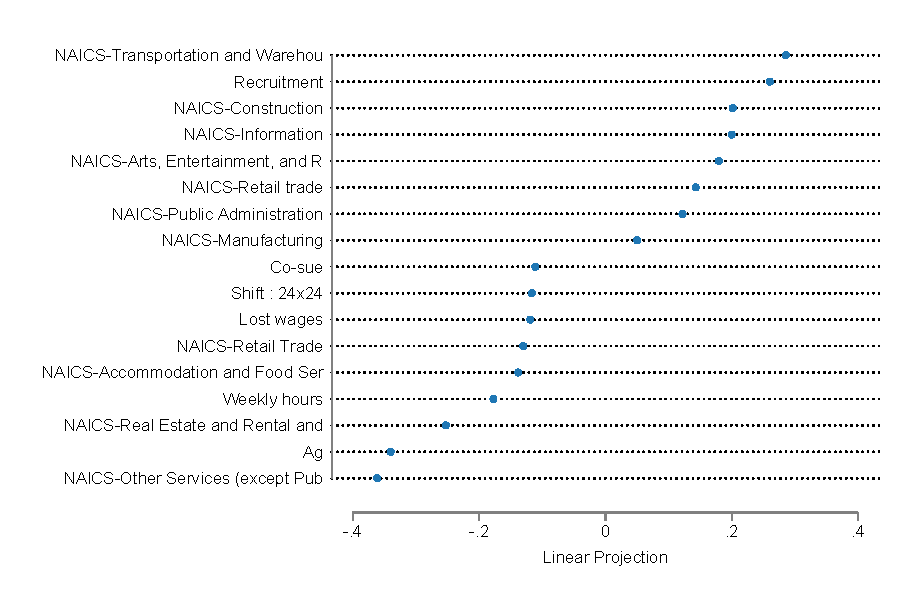
\includegraphics[width=\textwidth]{paper/Figures/coef1_m1.pdf}
    \end{subfigure}
    \begin{subfigure}{0.475\textwidth}
        \caption{Losing court ruling}
        \centering
        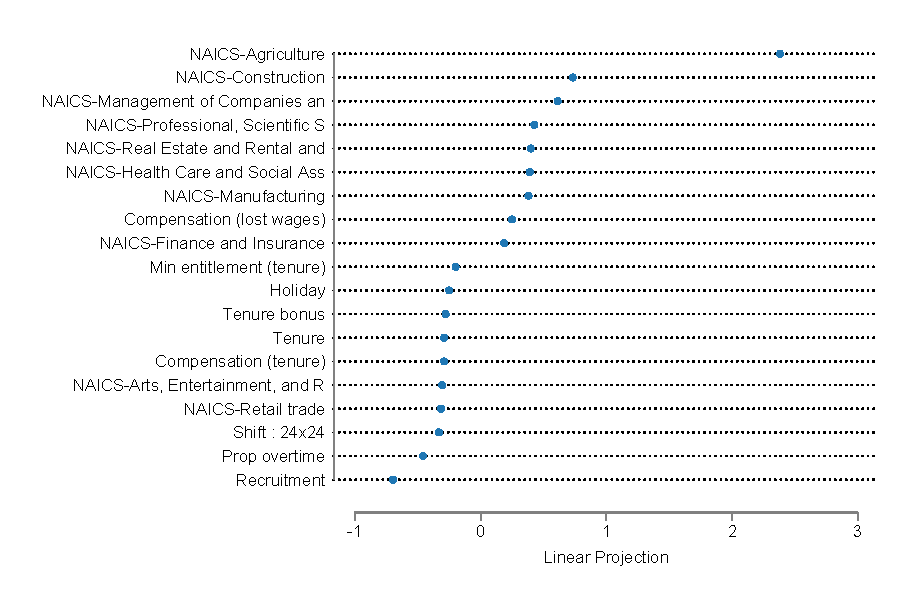
\includegraphics[width=\textwidth]{paper/Figures/coef1_m2.pdf}
    \end{subfigure}
    \begin{subfigure}{0.475\textwidth}
        \caption{Winning court ruling}
        \centering
        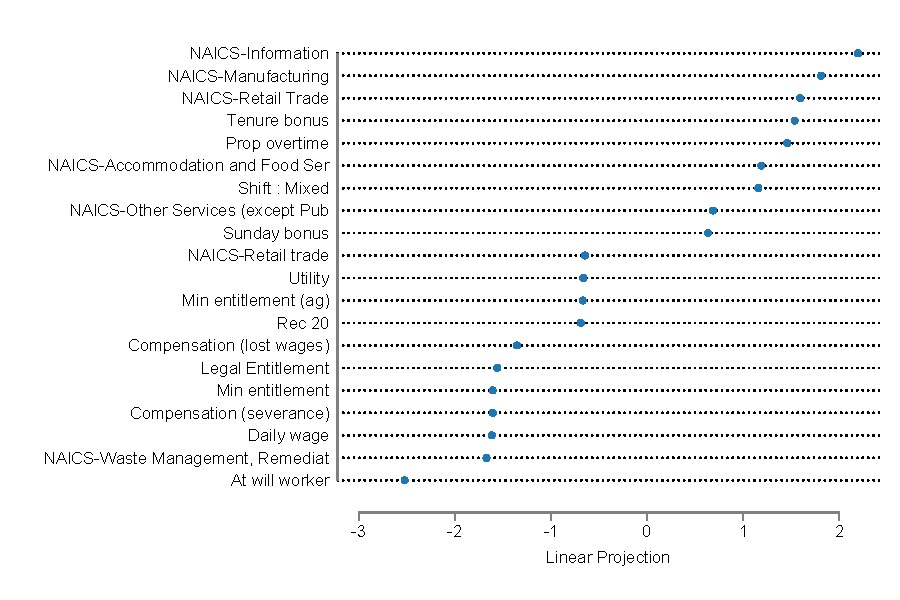
\includegraphics[width=\textwidth]{paper/Figures/coef1_m3.pdf}
    \end{subfigure}
    \begin{subfigure}{0.475\textwidth}
        \caption{Drop}
        \centering
        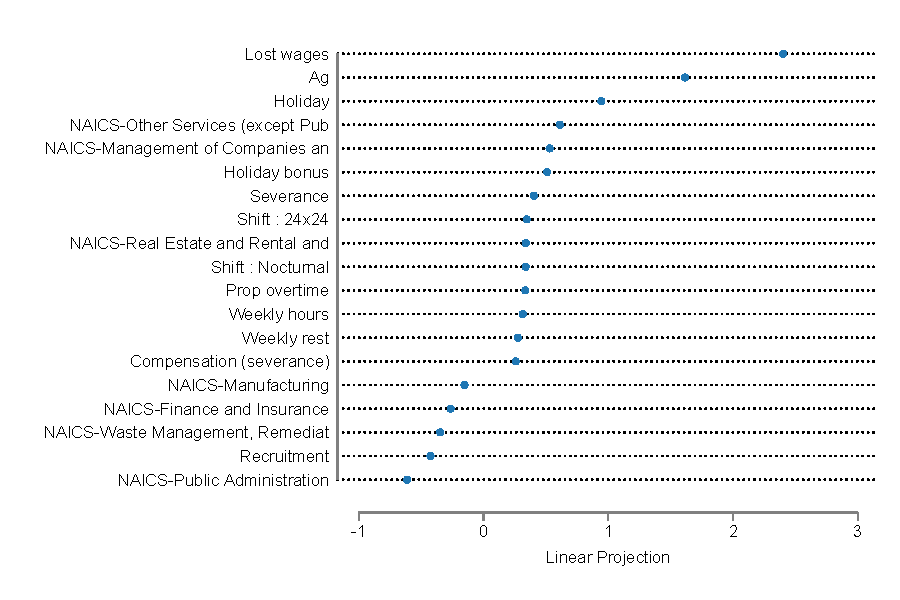
\includegraphics[width=\textwidth]{paper/Figures/coef1_m4.pdf}
    \end{subfigure}  
    \begin{subfigure}{0.475\textwidth}
        \caption{Winning on court ruling (Phase 2 \& 3)}
        \centering
        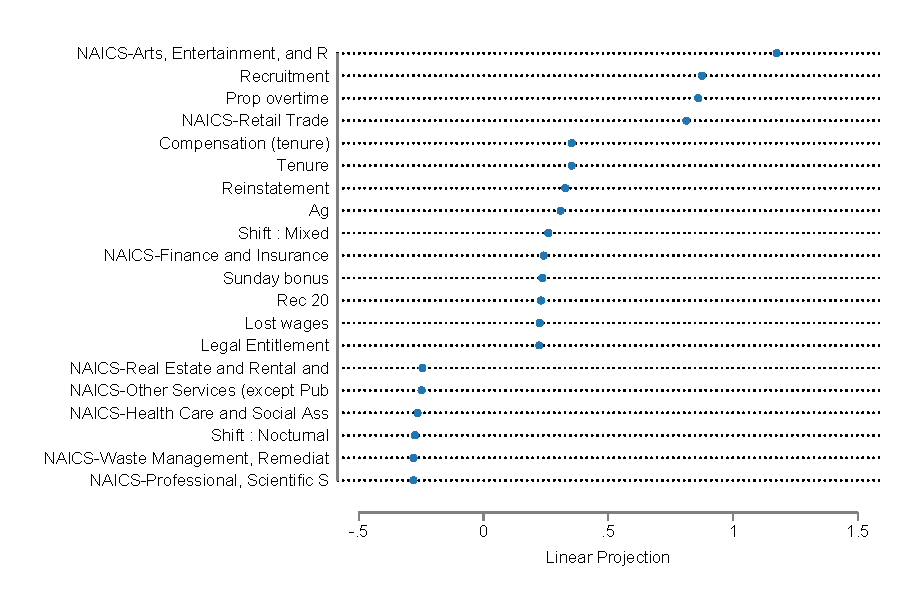
\includegraphics[width=\textwidth]{paper/Figures/coef1_m5.pdf}
    \end{subfigure}      
    \end{center}
     \scriptsize   This figure shows the main features and the role they play in each of the above models. We estimate the effect of this features on the predictions made by this models : $\log{\widehat{pr_i}} = \alpha + \beta_j \log{X_{i,j}} + \epsilon$. Note that we are leaving out all but the variable in question. Qualitatively, these betas can be used to assess the elasticity of the prediction function with the features, they can be interpreted as the elasticity of the partial effect of variable $X_{j}$ on the model's prediction. We only plot the 20 (out of 72) most important features defined as the ones with the biggest estimates in absolute value.   
          %\footnotesize{ \textit{Do file: }  \texttt{coefplots.do}}
\end{figure}






\subsection*{Continuous outcome variables}
Several relevant outcomes are continuous variables. We focus on three continuous variables to be provided to the parties: 

\begin{enumerate}
\item \textit{Amount collected conditional on a positive payment:} This is the peso amount actually collected by the plaintiff in the each of the two outcomes where they payments are positive: settlement and judgment in favor of the plaintiff, with recovery. The other endings all result in zero payments. 
\item \textit{Probability of Positive Recovery:} From the historical data for each casefile we know if the worker in fact was paid a positive amount or not (i.e. won the case in the court ruling and could indeed collect, or settled and got a positive amount).
\item \textit{Duration of the case:} The number of months from the filing of the case to the date when it ended. As a significant share of the cases were not resolved by the end of 2015, we discuss censoring below.
\end{enumerate}

For the continuous outcomes, we estimated a set of four different models for each of the two prediction problems.\footnote{Considering both regular and logarithmic models that would be eight different models for each outcome. The logarithmic models help to tackle the skewness of our dependent variable.} The four models were: (a) OLS regression, (b) GLM Boosting, (c) Random Forest\footnote{We perfomed grid search in order to find the best hyperparameter setting. We compared 7 different models with the number of trees ranging between 900 and 1500. Our final model resulted in a Random Forest of 1200 CARTs, which yielded an 86\% accuracy rate on test classification.}, (d) Ridge Regression\footnote{This was done with the libraries in R: e1071, randomForest, neuralnet, caTools, mboost.} \footnote{We also run the OLS and Random Forest models using logged data. In phase 2, we changed the models we estimated to include Kernel regression, running both OLS and Kernel in levels and logs. We do not present here the Boosted, Random Forest and Ridge regressions. The $corr(\hat{y^{j}},\hat{y^{k}})$ between the predicted values of model $j$ and model $k$ for the union of all models is above 0.8 for all models.}. As with the discrete variables, for each model the hyperparameters were chosen to minimize mean square error in the test set (MSE-T) using cross-validation. Once hyperparameters for each model were chosen, we chose among those optimized models based on their Mean Absolute Percentage Deviation (MAPD). 

Finally we also wanted to predict the duration of the trial from initial suit to termination. We used the data with models similar to those described for the amount collected. However, for phase 2 the predictions from these models were very noisy: the models could not beat a simple average within each type of ending, so we decided to present the simple average within each type of termination rather than a model as a function of observables. 

As with the discrete outcomes, Table \ref{ml_models_comparison_cont} shows the accuracy rate for settlement and duration outcomes and for each of the six models, highlighting in grey the ones chosen. The correlations range from 0.61 to 0.76 for the models selected for total compensation, but from 0.08 to 0.93 for the five duration outcomes. 
\\


\begin{landscape}
\begin{center}
  \begin{table}[H]
     \caption{Fit assessment of continuous calculator models}
     \label{ml_models_comparison_cont}
 \begin{subtable}{0.85\textwidth}
     \caption*{Phase 1: Continuous outcomes}
     \raggedleft
     \scriptsize{\begin{tabular}{lccccccc}
\toprule
 Ending type & N & Regression & Log-regression & Boosted regression & Random Forest & Log-Random Forest & Ridge Regression \\ 
\midrule
\midrule
\multicolumn{8}{c}{Total Compensation} \\ 
\midrule
Settlement  & 1236 & 0.61 & 0.55  & 0.61 & 0.63 & \cellcolor[rgb]{ .929,  .929,  .929} 0.61 & 0.61  \\
Court Ruling   & 66   & 0.70 & \cellcolor[rgb]{ .929,  .929,  .929} 0.76  & 0.70 & 0.49 & 0.28  & 0.67  \\ 
\midrule
\multicolumn{8}{c}{Duration} \\ 
\midrule
Settlement  & 1236 & 0.07 & 0.07  & \cellcolor[rgb]{ .929,  .929,  .929} 0.08 & 0.05 & 0.07   & 0.07  \\
Losing court ruling  & 49   & \cellcolor[rgb]{ .929,  .929,  .929} 0.93 & 0.94  & 0.93 & 0.87 & 0.81   & 0.93  \\
Winning court ruling & 66   & 0.64 & 0.65  & 0.64 & 0.47 & 0.44   & \cellcolor[rgb]{ .929,  .929,  .929} 0.65  \\
Expiry & 118  & 0.35 & 0.34  & \cellcolor[rgb]{ .929,  .929,  .929} 0.37 & 0.29 & 0.39   & 0.42  \\
Drop   & 468  & 0.20 & 0.16  & 0.19 & 0.13 & \cellcolor[rgb]{ .929,  .929,  .929} 0.17   & 0.05 \\
\bottomrule 
\end{tabular}
}
 \end{subtable}%
   
     \bigskip
 \begin{subtable}{1\textwidth}
       \centering
         \caption*{Phases 2 and 3: Continuous outcomes}
         \scriptsize{\begin{tabular}{lccccc}
\toprule
  Ending type  & N & Regression & Kernel regression & Log-regression & Log-kernel regression \\
\midrule
\midrule
\multicolumn{6}{c}{Total Compensation} \\ 
\midrule
Settlement   & 3130 & 0.59    & 0.46     &  \cellcolor[rgb]{ .929,  .929,  .929} 0.69     & 0.63     \\
Court ruling & 105  & \cellcolor[rgb]{ .929,  .929,  .929} 0.44    & 0.30     & 0.18     & -0.06   \\
\bottomrule
\end{tabular}}
 \end{subtable}
 
  \scriptsize
   \textit{Notes:} Some statistics on the predictive power of the models considered for both -Phase 1 and Phase 2- calculator calibration processes. Statistics for models chosen for each problem are shown in bold. We show $Corr(y, \hat{y})$ for continuous outcomes. We considered random forests both for continuous and categorical outcome variables, using the algorithm's regression and classification methods, respectively.
%     \textit{RScripts: } \texttt{calc\_predictions.R}
 \end{table}
 \end{center}
\end{landscape}


\begin{figure}[H]
    \caption{Variable importance for continuous models (total compensation)}
    \label{}
    \begin{center}
    \begin{subfigure}{0.475\textwidth}
        \caption{Settlement}
        \centering
        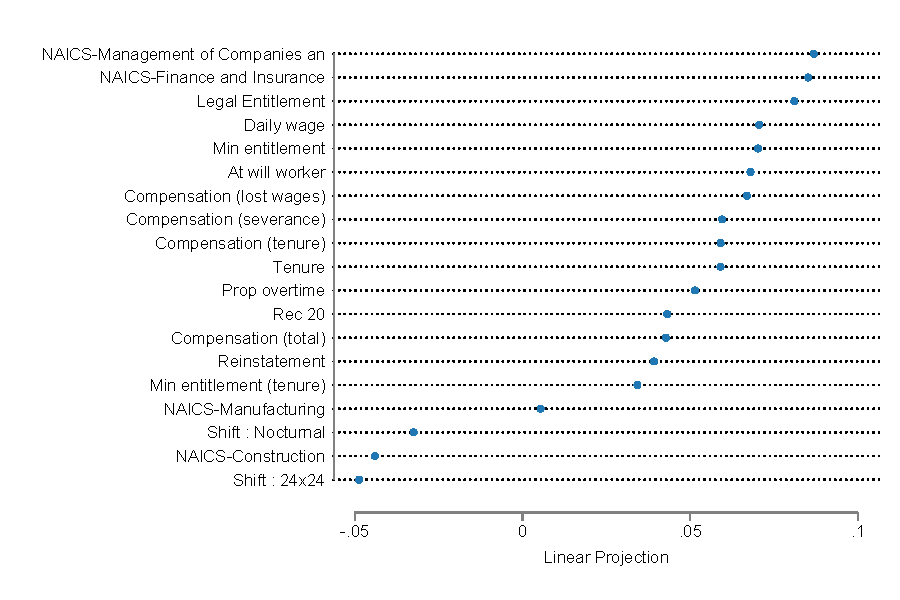
\includegraphics[width=\textwidth]{paper/Figures/coef1_m6.pdf}
    \end{subfigure}
    \begin{subfigure}{0.475\textwidth}
        \caption{Court ruling}
        \centering
        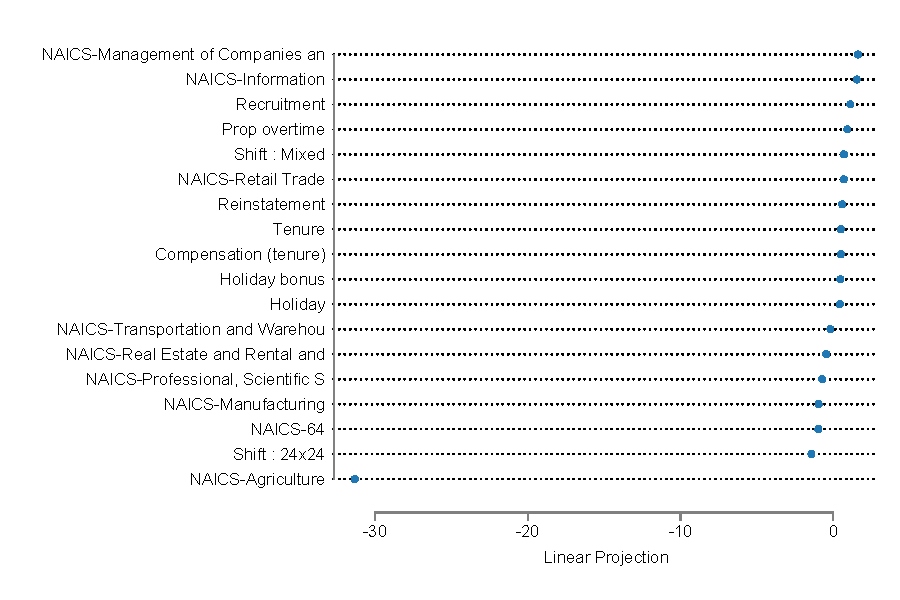
\includegraphics[width=\textwidth]{paper/Figures/coef1_m7.pdf}
    \end{subfigure}
   \begin{subfigure}{0.475\textwidth}
        \caption{Settlement (Phase 2 \& 3)}
        \centering
        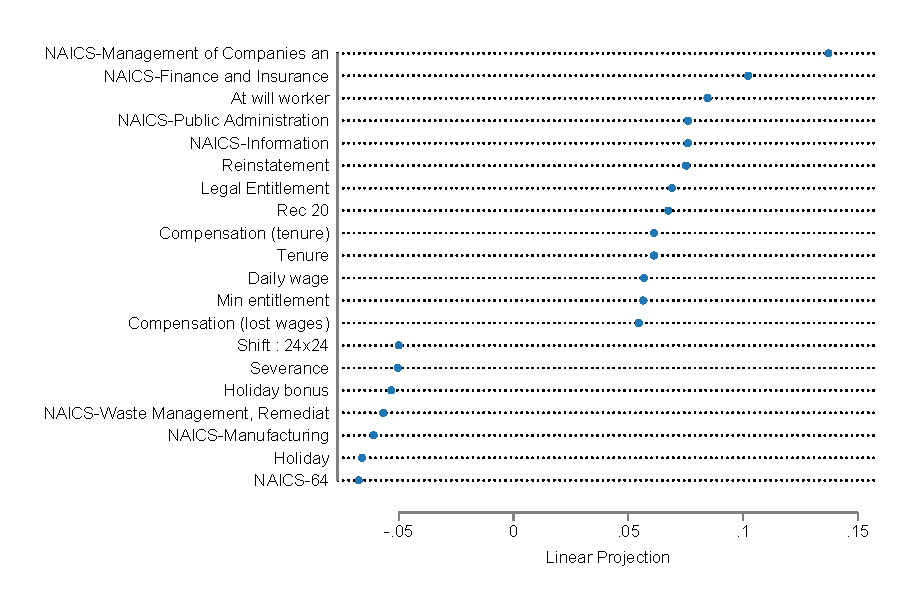
\includegraphics[width=\textwidth]{paper/Figures/coef1_m8.pdf}
    \end{subfigure}
    \begin{subfigure}{0.475\textwidth}
        \caption{Court ruling (Phase 2 \& 3)}
        \centering
        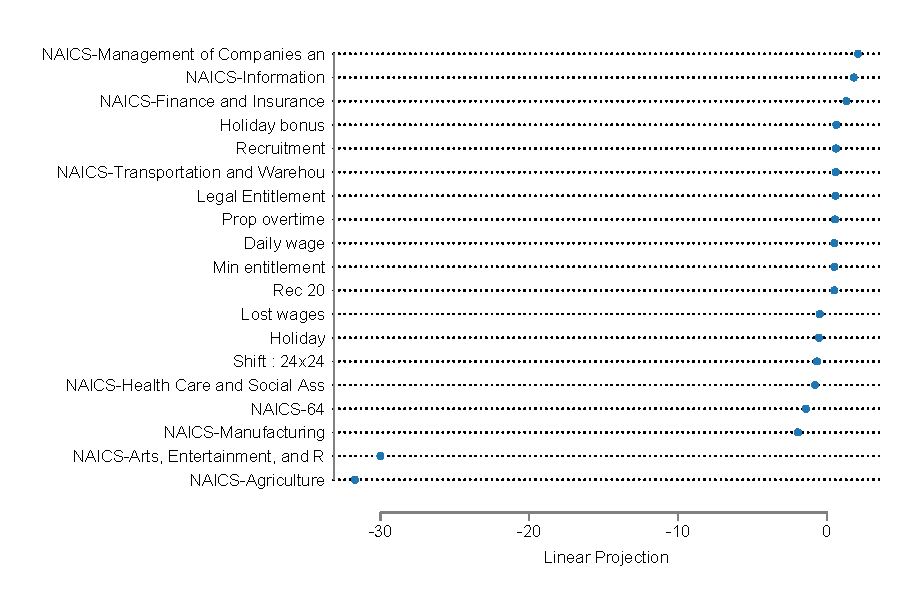
\includegraphics[width=\textwidth]{paper/Figures/coef1_m9.pdf}
    \end{subfigure}     
    \end{center}
     \scriptsize   This figure shows the main features and the role they play in each of the above models. We estimate the effect of this features on the predictions made by this models : $\log{\widehat{pr_i}} = \alpha + \beta_j \log{X_{i,j}} + \epsilon$. Note that we are leaving out all but the variable in question. Qualitatively, these betas can be used to assess the elasticity of the prediction function with the features, they can be interpreted as the elasticity of the partial effect of variable $X_{j}$ on the model's prediction.
     We only plot the 20 (out of 72) most important features defined as the ones which exhibit the higher correlation in absolute value. 
          %\footnotesize{ \textit{Do file: }  \texttt{coefplots.do}}
\end{figure}




\begin{figure}[H]
    \caption{Variable importance for continuous models (duration)}
    \label{PredictorsCont2}
    \begin{center}
    \begin{subfigure}{0.475\textwidth}
        \caption{Settlement}
        \centering
        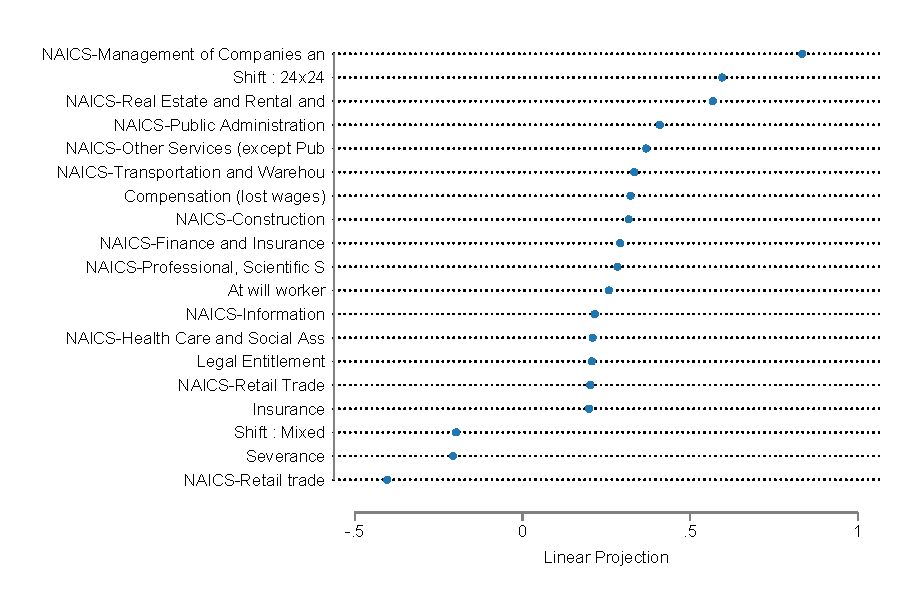
\includegraphics[width=\textwidth]{paper/Figures/coef1_m10.pdf}
    \end{subfigure}
    \begin{subfigure}{0.475\textwidth}
        \caption{Losing court ruling}
        \centering
        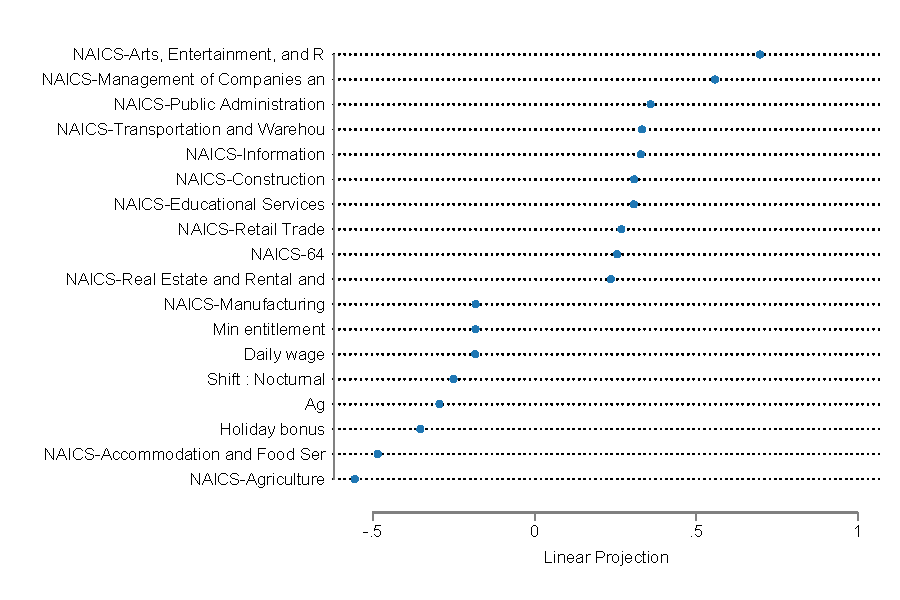
\includegraphics[width=\textwidth]{paper/Figures/coef1_m11.pdf}
    \end{subfigure}
   \begin{subfigure}{0.475\textwidth}
        \caption{Winning court ruling}
        \centering
        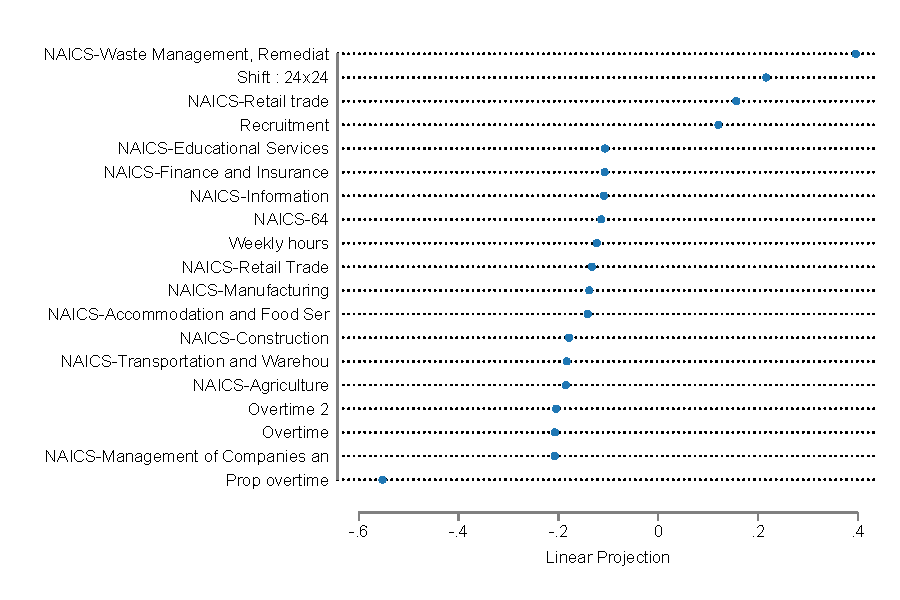
\includegraphics[width=\textwidth]{paper/Figures/coef1_m12.pdf}
    \end{subfigure}
    \begin{subfigure}{0.475\textwidth}
        \caption{Expiry }
        \centering
        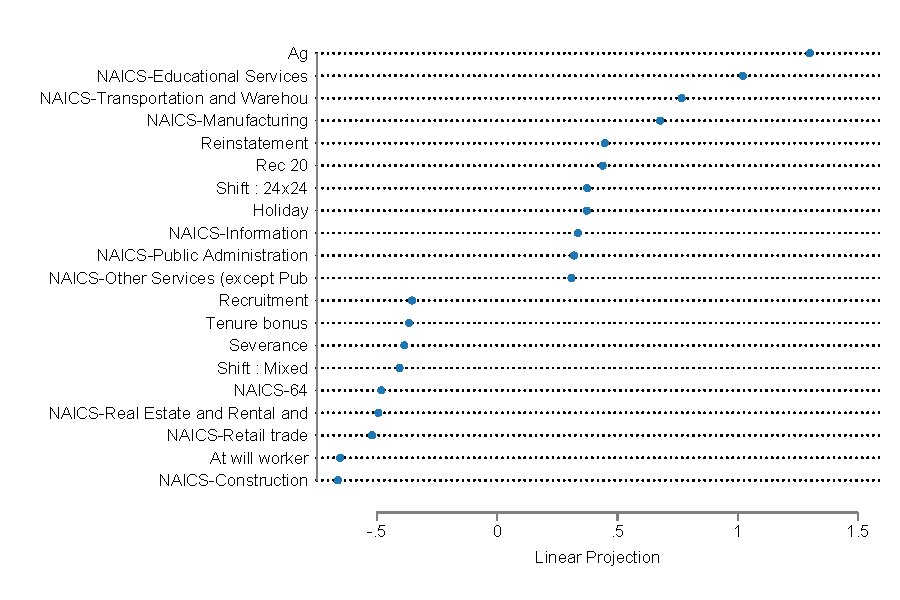
\includegraphics[width=\textwidth]{paper/Figures/coef1_m13.pdf}
    \end{subfigure}     
        \begin{subfigure}{0.475\textwidth}
        \caption{Drop }
        \centering
        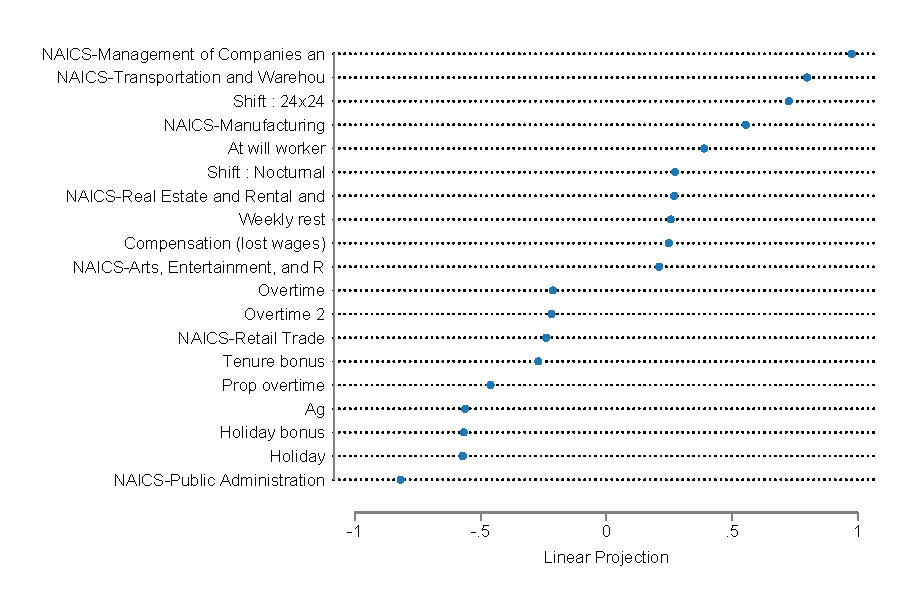
\includegraphics[width=\textwidth]{paper/Figures/coef1_m14.pdf}
    \end{subfigure}     
    \end{center}
     \scriptsize This figure shows the main features and the role they play in each of the above models. We estimate the effect of this features on the predictions made by this models : $\log{\widehat{pr_i}} = \alpha + \beta_j \log{X_{i,j}} + \epsilon$. Note that we are leaving out all but the variable in question. Qualitatively, these betas can be used to assess the elasticity of the prediction function with the features, they can be interpreted as the elasticity of the partial effect of variable $X_{j}$ on the model's prediction.  We only plot the 20 (out of 72) most important features defined as the ones with the biggest estimates in absolute value.  
          %\footnotesize{ \textit{Do file: }  \texttt{coefplots.do}}
\end{figure}


\subsection*{Other issues: Censoring}

All of the models are estimated on a sample of cases filed in 2011 and completed by the end of 2015. The fact that the sample contains only the cases that were resolved could introduce a bias in the prediction of outcomes of ongoing cases. For example, if we are interested in the probability of winning \textit{eventually} and if cases with larger expected payouts take longer to resolve, then excluding the unresolved cases may produce an underestimate of the average payments in all cases.  

We are aware of this bias and it was communicated to the parties when the calculator information was provided. Although we cannot know how large the bias is, we performed two exercises that suggest it is not large. First, we compare characteristics of ongoing cases with those of the historical cases used in the models. In Figure \ref{covariate_distribution} we show that the two sets of cases are similar. The second exercise compares the characteristics of completed and continuing lawsuits within the historical data. To do this we drew a random sample of 956 cases filed in 2011 that were not finished by 2015 (i.e. this represents the complement of our historical dataset). We compare these 956 cases to the completed cases used to develop the models. Figure \ref{FinishedUnfinished} reports the results. There are no significant differences between these two samples, and the magnitude of the measured differences are all very small. 

\begin{figure}[H]
\caption{Covariate distribution comparison : Historical and Phase 1 data}
\label{covariate_distribution}
    \begin{center}
        \begin{subfigure}{0.7\textwidth}
            \caption*{Continuous variables}
            \centering
            \includegraphics[width=0.7\textwidth]{paper/Figures/covariates_continous.tiff}
        \end{subfigure}
        \begin{subfigure}{0.7\textwidth}
            \caption*{Categorical variables}
            \centering
            \includegraphics[width=0.7\textwidth]{covariates_categorical.tiff}
        \end{subfigure}
        \end{center}
          {\scriptsize \textit{Notes: } Covariate distributions comparisons. We compare between -used to calibrate our calculator- and Phase 1 data.  All continuous variables are plotted in logs. Color guide is the same for both variable types. Plots for continuous variables show the p-value of a Kolmogorov–Smirnov test in the subtitle. In the categorical covariates plot, we show significance of a two-sided t-test of differences in means between samples.}
    % {\scriptsize \textit{Script: } \texttt{covariate\_plots.R , covariate\_plots\_hd.R }}
        \end{figure}
        
        
 \begin{figure}[H]
        \caption{Covariate distribution comparison : Historical data: Ended and not ended cases}
        \label{FinishedUnfinished}
        \begin{center}
             \begin{subfigure}{\textwidth}
            \caption*{Continuous variables}
            \centering
            
\includegraphics[width=0.7\textwidth]{covariates_hdsample_continous.PNG}
        \end{subfigure}
        \begin{subfigure}{0.7\textwidth}
            \caption*{Categorical variables}
            \centering
            \includegraphics[width=0.7\textwidth]{covariates_hdsample_categorical.tiff}
        \end{subfigure}
    \end{center}
    {\scriptsize \textit{Notes: } Covariate distributions comparisons between historical data cases: ended and not ended after 3 years. All continuous variables are plotted in logs. Color guide is the same for both variable types. Plots for continuous variables show the p-value of a Kolmogorov–Smirnov test in the subtitle. In the categorical covariates plot, we show significance of a two-sided t-test of differences in means between samples.}
    % {\scriptsize \textit{Script: } \texttt{covariate\_plots.R , covariate\_plots\_hd.R }}
\end{figure}


%\begin{figure}[!ht]
%    \caption{Compensation histograms - Historical Data}
%    \label{hist_npv_hd}
%    \begin{center}
%        
\includegraphics[width=0.5\textwidth]{hist_npv_hd.pdf}
%        \end{center}
%        {\scriptsize \textit{Notes:} Distribution of compensation %in present value at the time of suing with a monthly %interest rate of $3.43$, with a $30$ percent cost, and an %initial fee of MXN\$2000 pesos for private lawyers and %deflated into June 2016 pesos. }
%        % \textit{Do File: } \texttt{histograms\_npv\_hd.do}
%\end{figure}

